\paragraph*{2.3 Обратная задача кинематики}$\phantom{-}$\\
\hspace*{\parindent}Обратная задача кинематики (или обобщенно ОЗК) заключается в определение обобщенных координат через линейные и угловые координаты рабочего инструмента (хвата). \\

\hspace*{\parindent}Рассмотрим аналитический (геометрический) метод расчёта обобщенных коэффициентов системы:\\
\begin{enumerate} 
\item[1.]  В начале рассмотрим схему, которая была получена после присвоения каждому звену системы координат и определения углов вращения каждого из них\\

\begin{center}
    \includegraphics[width=0.9\textwidth]{axesIK.jpg}\\
    Рисунок 2.3.1 схема манипулятора с обозначенными осями и углами вращений.\\
\end{center}

\item[2.] Далее рассмотрим вид сверху для данной системы\\

\begin{center}
    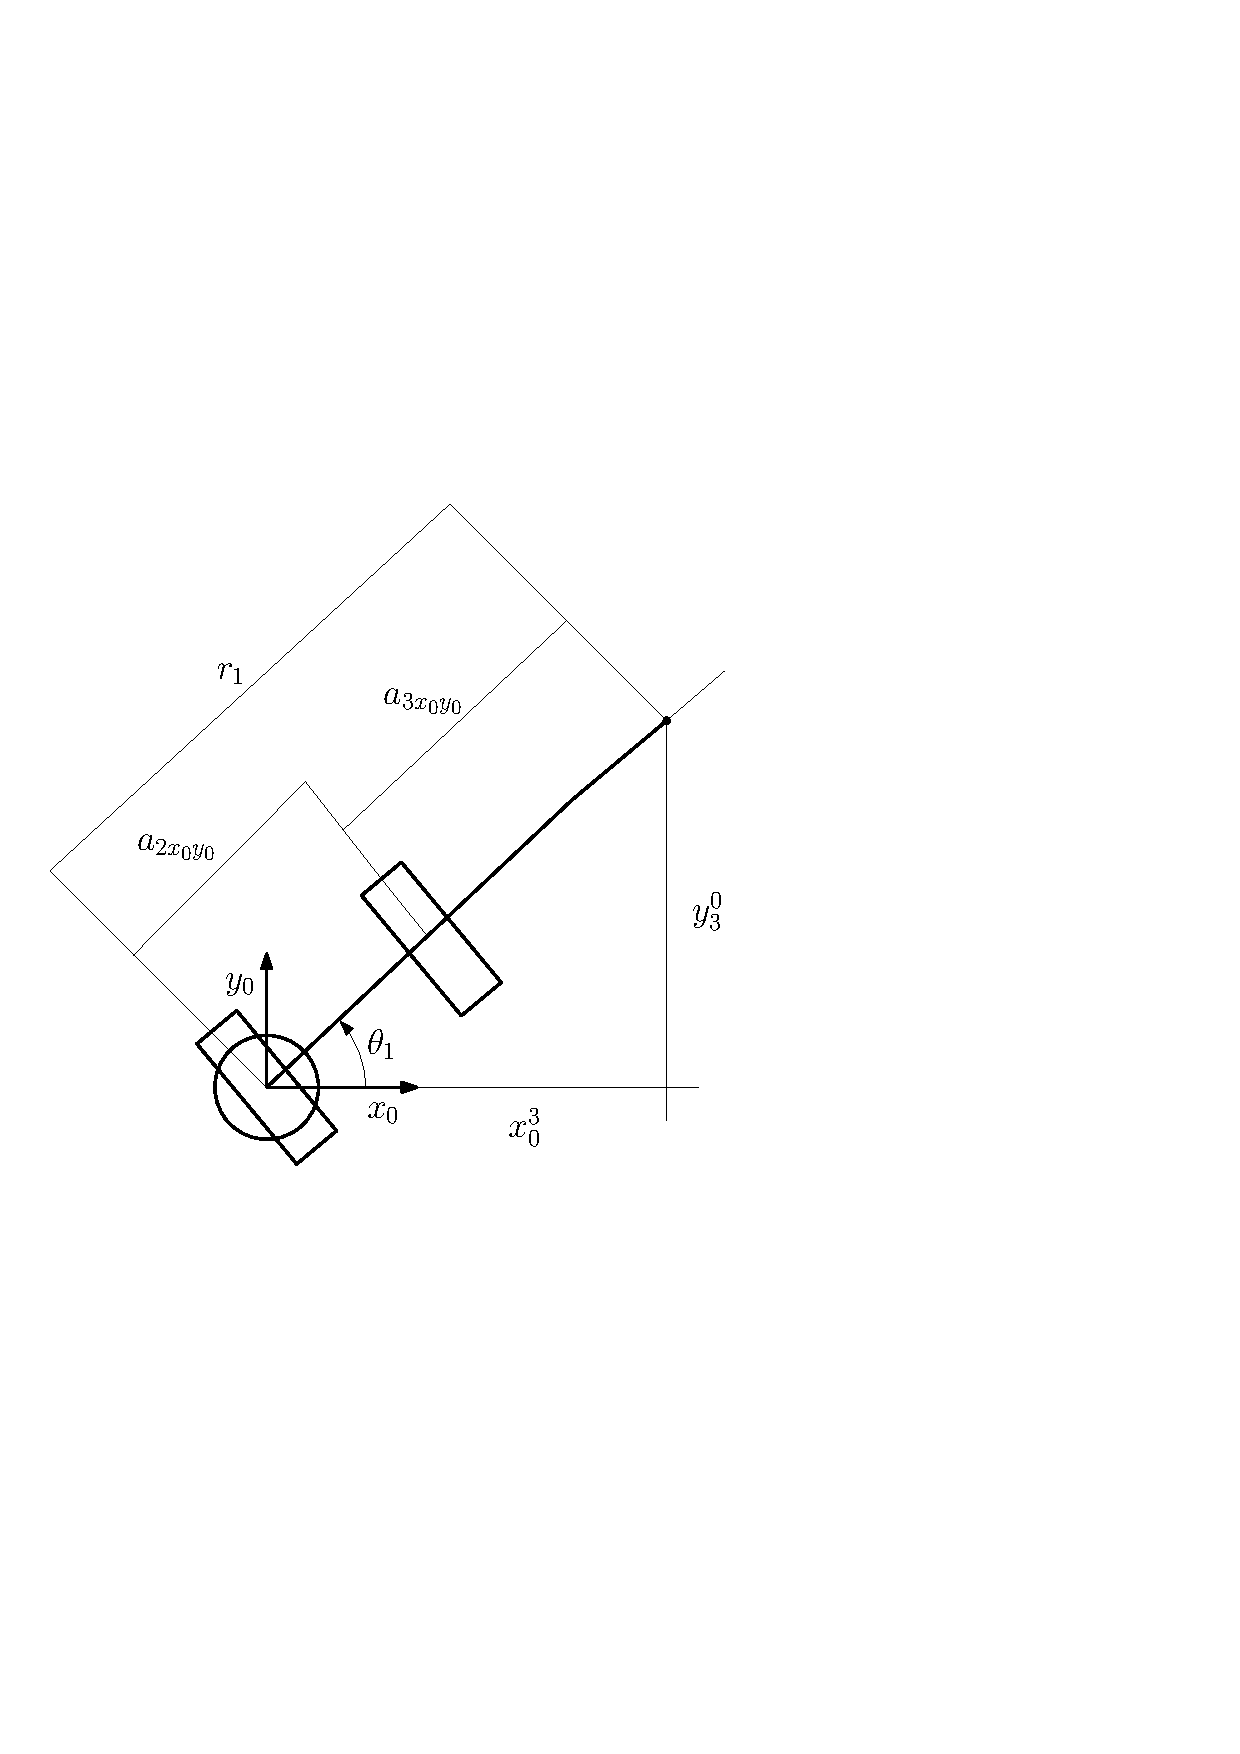
\includegraphics[width=0.5\textwidth]{2.pdf}\\
     Рисунок 2.3.2 Вид схемы сверху (проекция $x_0 y_0$).\\
\end{center}


Обозначим нулевую систему координат и угол вращения $\theta_1$ (можно было бы ещё обозначить известные параметры $a_2$ и  $a_3$, но в данной проекции отображаются $но в данном случае мы наблюдаем лишь их проекции. (мне кажется больше в скобках ничего не нужно)$не явные(известные) значения этих параметров, а их проекции на плоскость $x_0 y_0$, которые соответственно изменяются с изменениями угла, поэтому не указываются на таком виде). Можно заметить, что искомый угол $\theta_1$ выражается через отношение $y_3^0$ $x_3^0$ таким образом можно записать:$Можно заметить, что искомый угол можно выразить как$\\
$$\theta_1=arctg(\frac{y_3^0}{x_3^0});$$

\item[3.] Далее рассмотрим вид спереди данной системы, придав звеньям некоторое смещение $Не уверен, но мне кажется что комментарии не нужны$(для более наглядного выражения углов). Тут можно выделить неоднозначность решения ОЗК, поскольку можно заметить, что прийти в данную точку возможно несколькими вариантами смещения, к примеру:\\

\begin{center}
    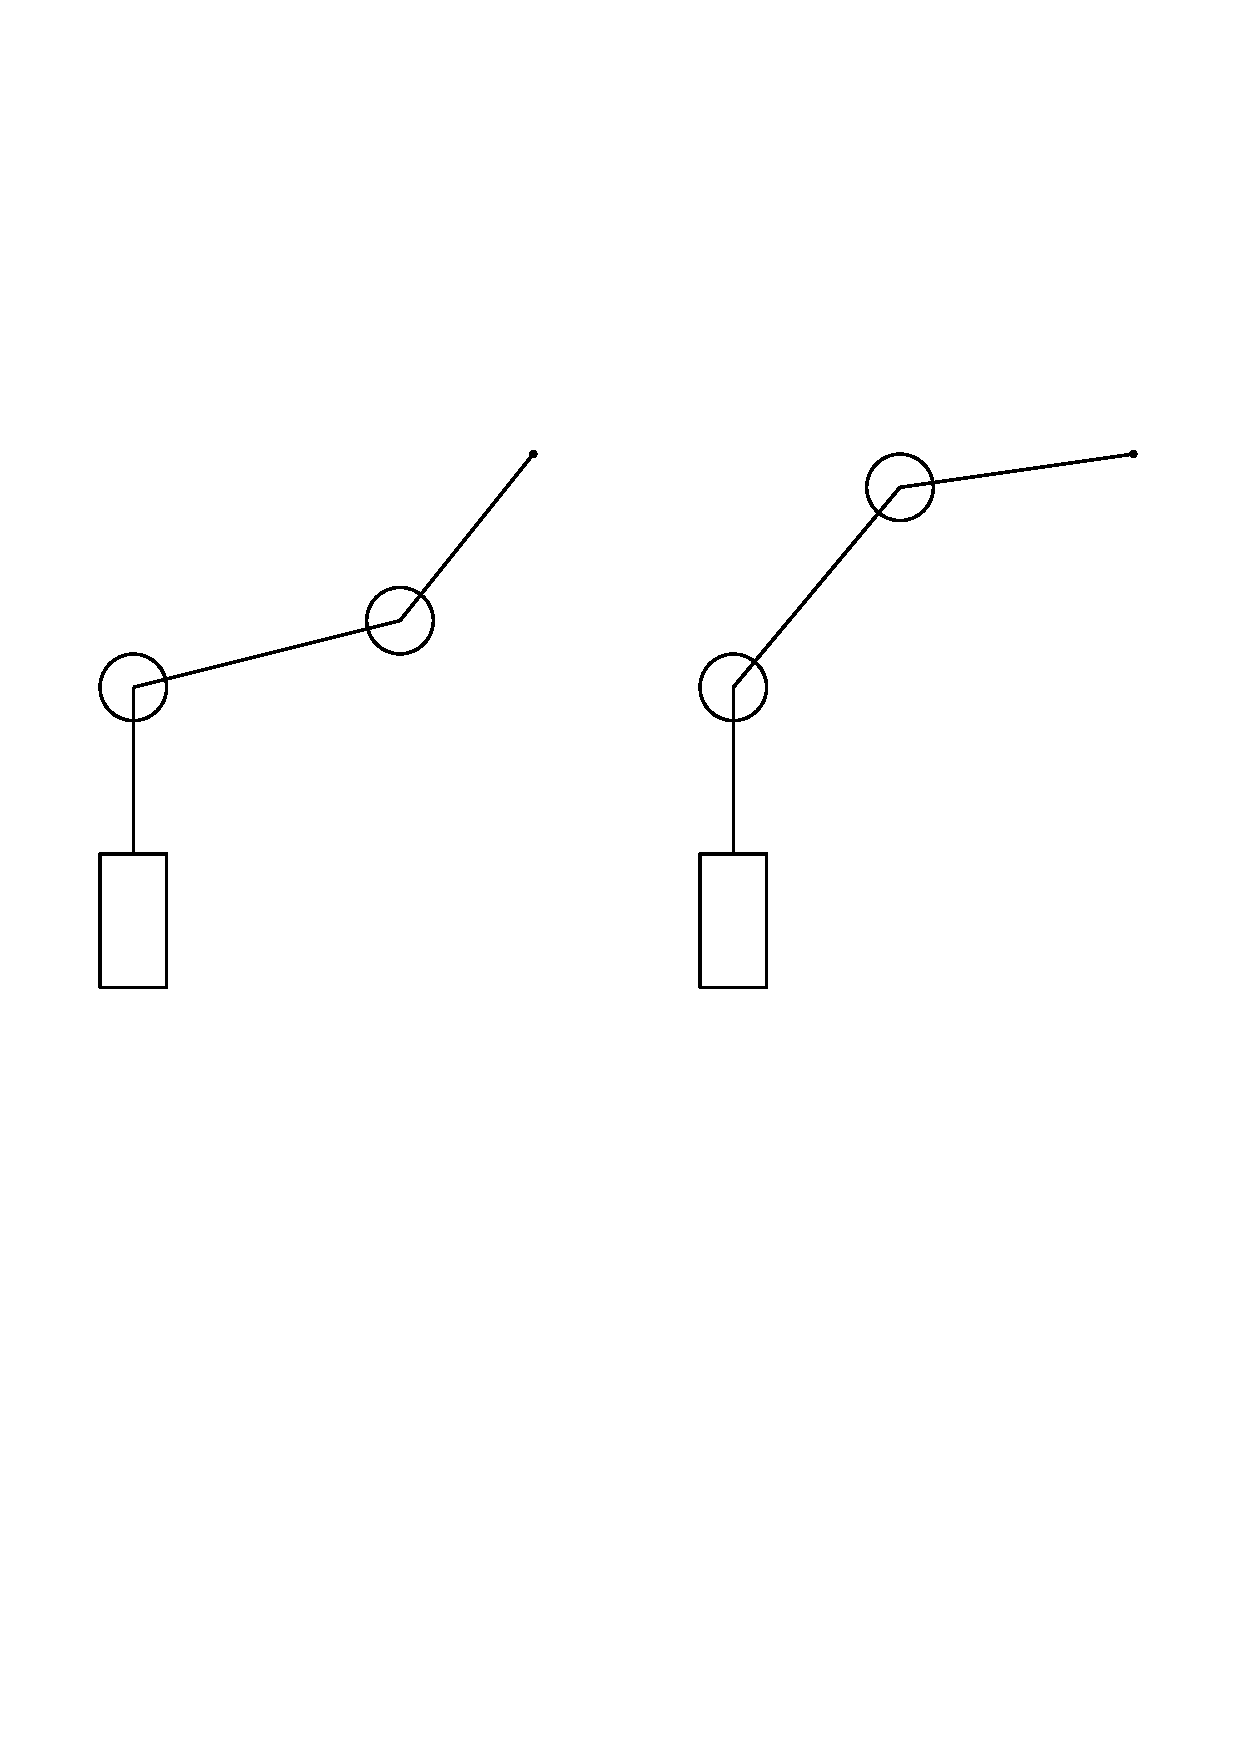
\includegraphics[width=0.55\textwidth]{1.pdf}\\
    а) Второе сочленение расположено снизу    б) Второе сочленение расположено сверху.\\
     Рисунок 2.3.3 схема манипулятора для некоторых одинаковых коэффициентов рабочего инструмента.\\
     $Рисунок 2.3.3 схема манипулятора для некоторых одинаковых коэффициентов рабочего инструмента.а) Второе сочленение расположено снизу, б) второе сочленение расположено сверху\\$%Вроде обычно так обозначают, либо в данном случае можно вообще без объяснения, если кратко то я могу ещё попридираться к этому
\end{center}
%Каждая конфигурация при решении ОЗК ограничивает рабочую облась, поэтому при решении задачи отдается предпочтение конфигурации которая в большей степени удовлетворяет достижению необходимой нам рабочей области.
Пусть будем рассматривать вариант с верхним расположением второго сочленения.\\%Для примера рассмотрим вариант ...
Итак, здесь помимо обозначения нулевой системы координат(можем обозначить только $z_1$, поскольку она является единственной не перпендикулярной осью вращения и задает своё изменение для $x_0$ и $y_0$) и углов вращения($\theta_2$ от оси,  $\theta_3$ от продолжения второго звена) можно обозначить параметры $d_1$, $a_2$ и $a_3$, поскольку их величины в данной проекции не изменяются. Также можно задать вспомогательные величины углов и длин: соединение первого и третьего сочленения $r_3$, достроение до треугольника $r_1$ и $r_2$, а также углы $\phi_1$, $\phi_2$, $\phi_3$.\\
%Мне кажется слишком много отступлений в скобочках, возможно я сейчас невыспавшийся злой и придираюсь, но я теряю мысль пока читаю отступления.

\begin{center}
    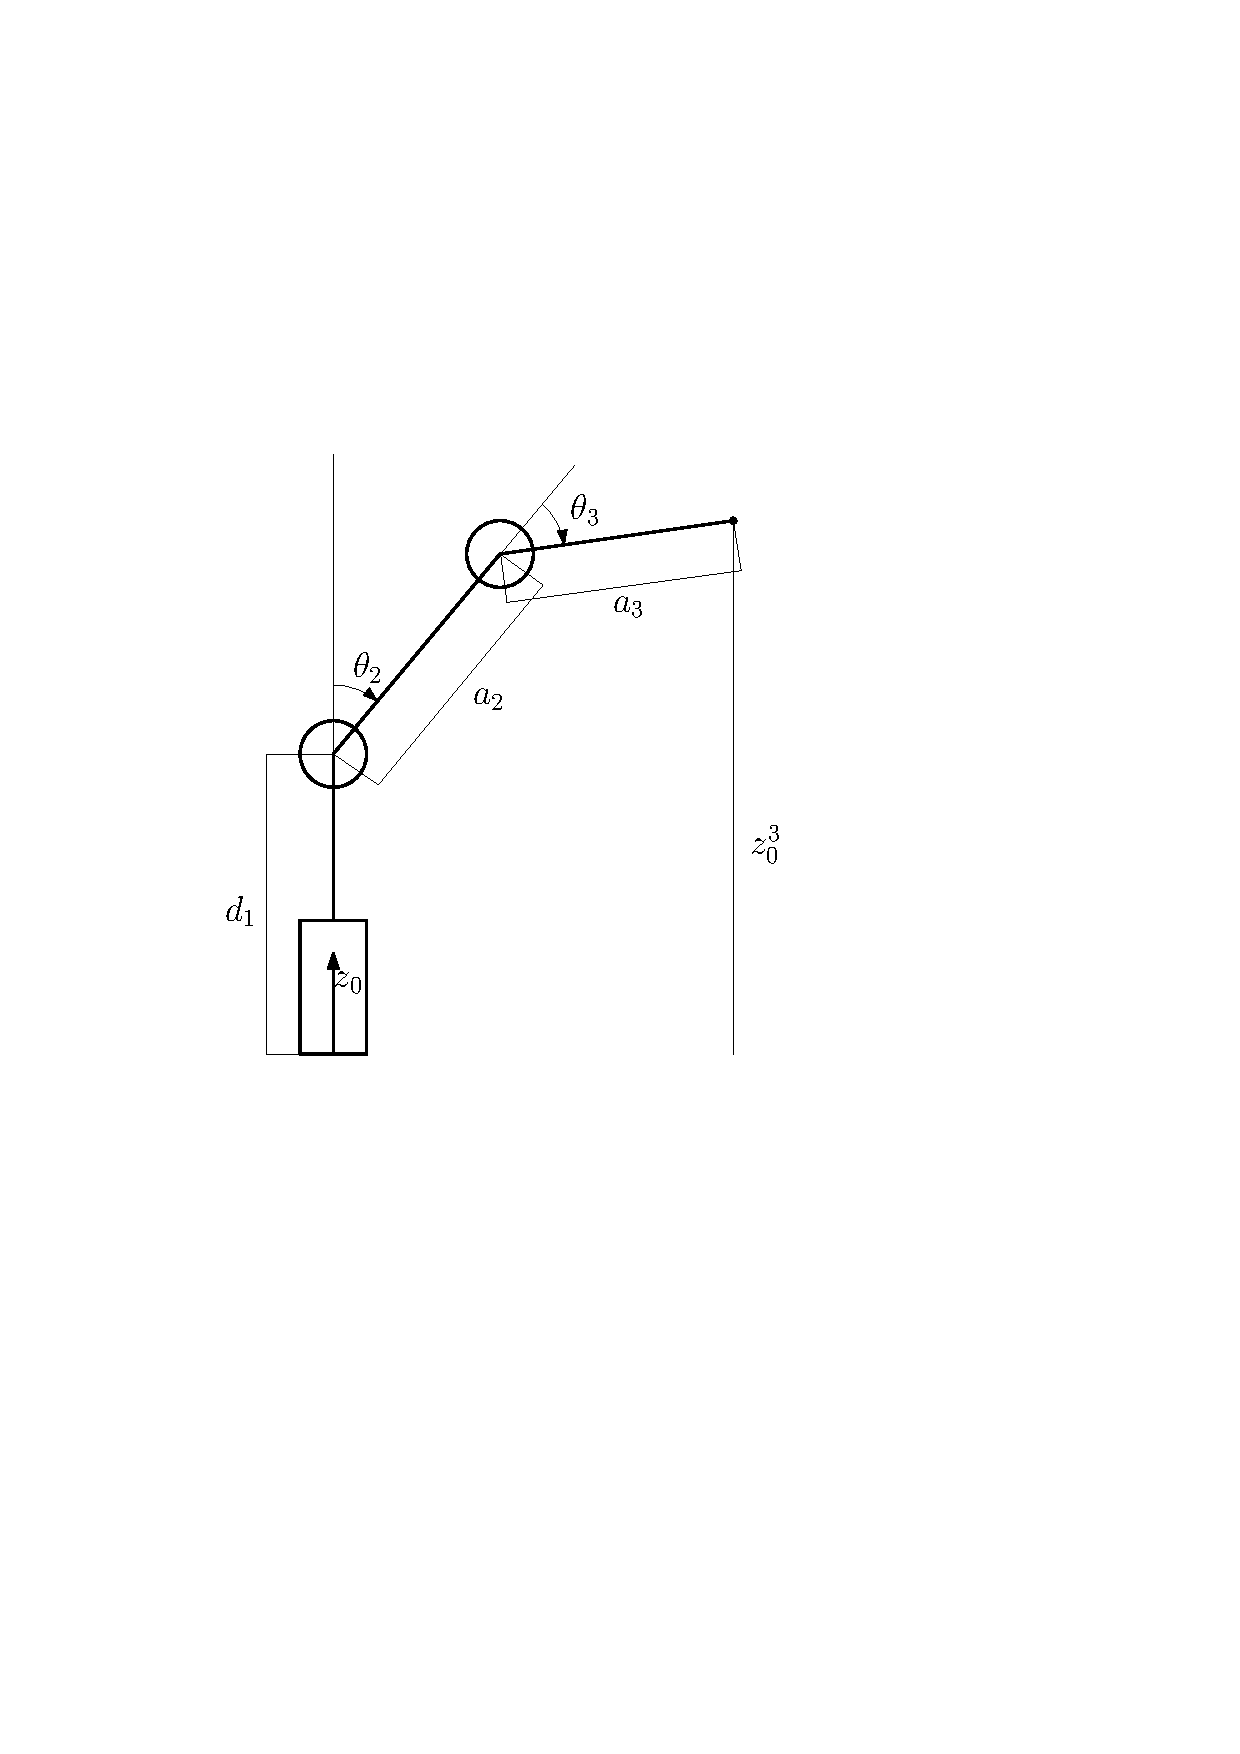
\includegraphics[width=0.4\textwidth]{3.pdf}\\
     Рисунок 2.3.4 Вид схемы спереди (проекция $x_0z_0$).\\
\end{center}

Рассмотрим поподробнее схему между вторым, третьим и инструментальным звеньями.\\

\begin{center}
    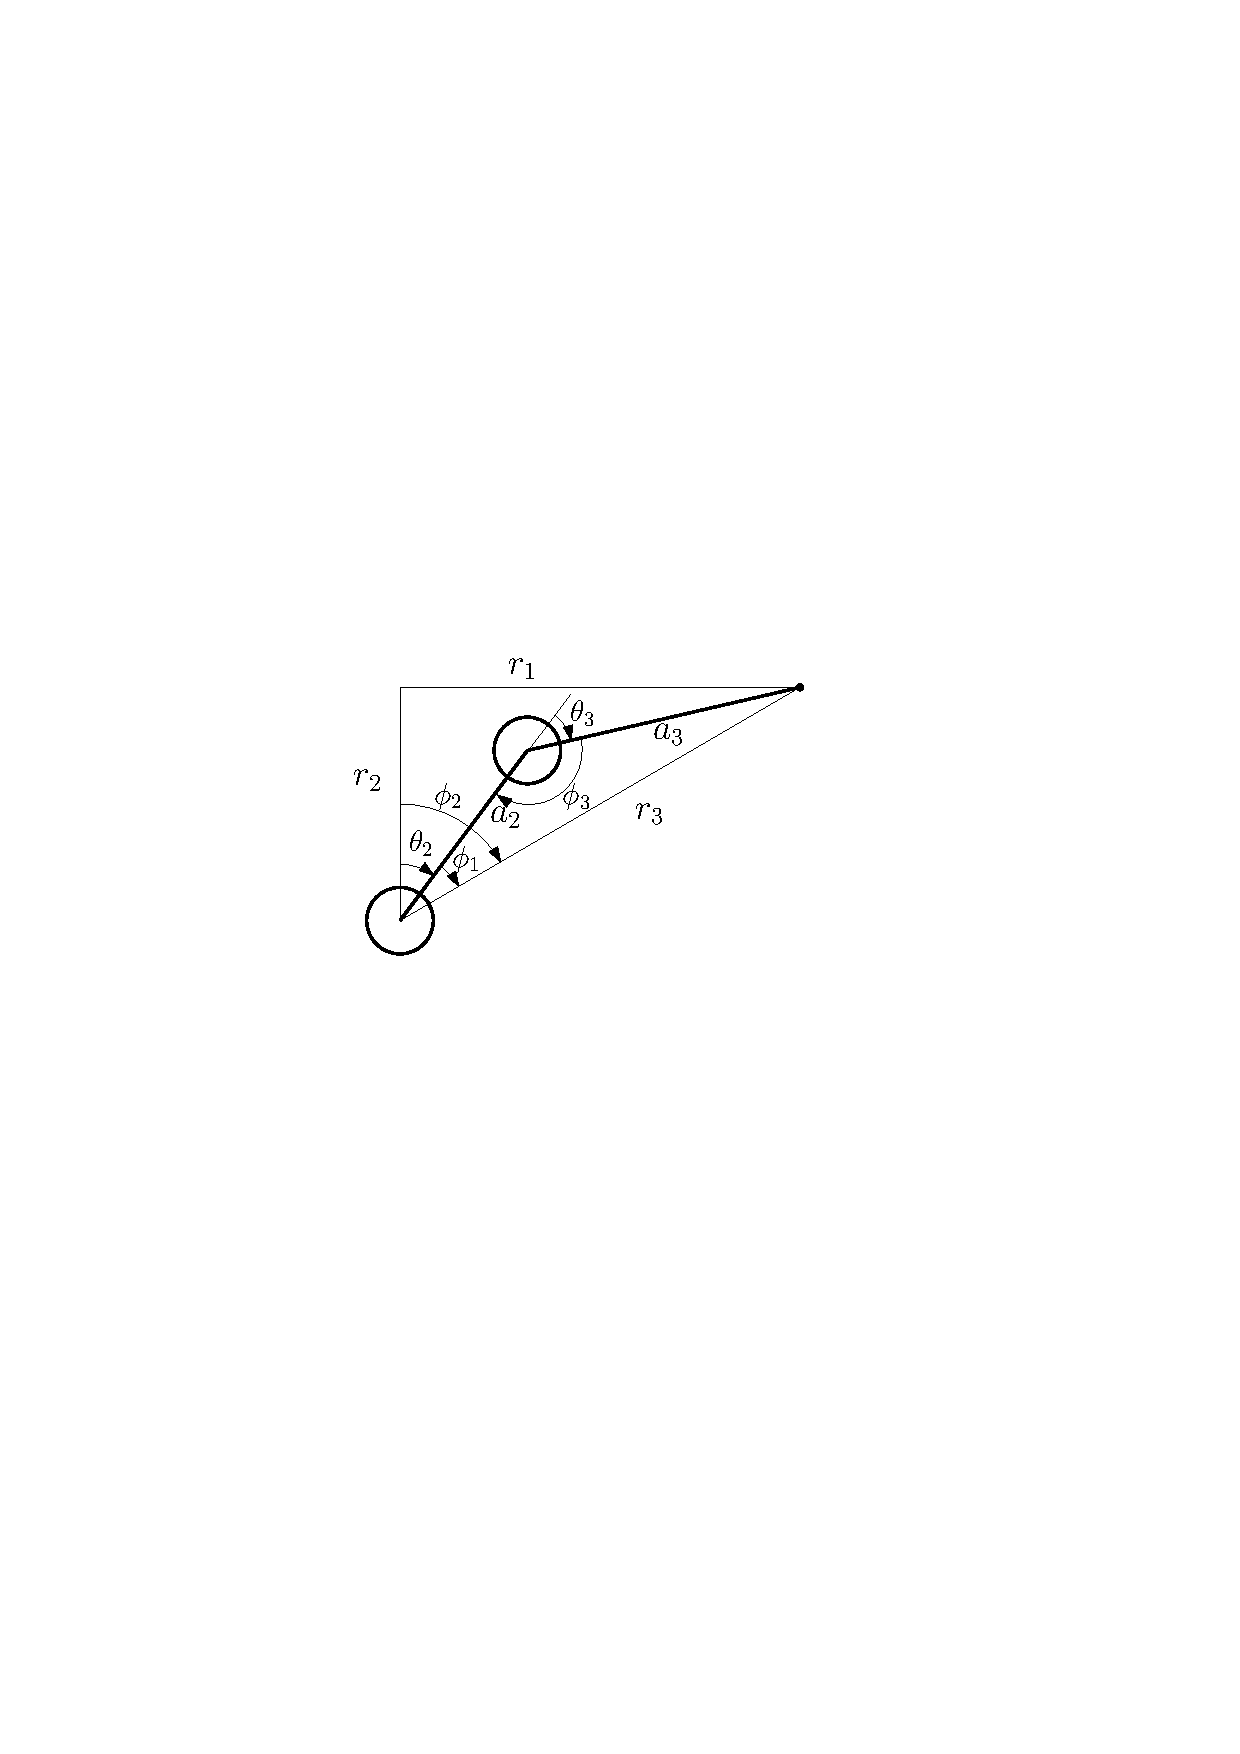
\includegraphics[width=0.5\textwidth]{4.pdf}\\
         Рисунок 2.3.5 Приближенное изображение схемы с необходимыми обозначениями. \\

\end{center}

Можно представить угол $\theta_2$ как разницу между углами $\phi_2$ и $\phi_1$:\\
$$\theta_2 = \phi_2 - \phi_1$$
- где $\phi_2$ видно из рисунка (треугольник, образованный сторонами $r_1$, $r_2$ и $r_3$ прямоугольный, $\phi_2$ определяет отношение катетов);
$$\phi_2 = arctg(\frac{r_1}{r_2})$$
- $r_2$ находится как разность между $z_0^3$ и $d_1$: \\
$$r_2=z_3^0 - d_1$$
- $r_1$ определяется из предыдущей проекции ($x_0y_0$) как сумма проекций $a_{2x0y0}$ $a_{3x0y0}$, которые в свою очередь определяются через теорему Пифагора:\\ $$r_1=a_{2x0y0}+a_{3x0y0}=\sqrt{(x_3^0)^2+(y_3^0)^2}$$
- $\phi_1$ находим через теорему косинусов в треугольнике, образованном сторонами $a_2$, $a_3$, $r_3$:\\
$$a_3^2 = a_2^2 + r_3^2 - 2 a_2 r_3 cos\phi_1$$
$$cos\phi_1 = \frac{a_2^2 + r_3^2 - a_3^2}{2 a_2 r_3} \rightarrow \phi_1 = arccos(\frac{a_2^2 + r_3^2 - a_3^2}{2 a_2 r_3})$$
- $r_3$ находится так же по теореме Пифагора:\\
%Вставить обозначения векторов
$$r_3=\sqrt{r_1^2+r_2^2}=\sqrt{(x_3^0)^2+(y_3^0)^2)+(z_3^0 - d_1)^2}$$
Таким образом получаем:\\
$$\theta_2=arctg(\frac{r_1}{r_2}) - arccos(\frac{a_2^2 + r_3^2 - a_3^2}{2 a_2 r_3})$$
$$ \theta_2=arctg(\frac{\sqrt{(x_3^0)^2+(y_3^0)^2}}{z_3^0-d_1}) - arccos(\frac{a_2^2 + ((x_3^0)^2+(y_3^0)^2)+(z_3^0 - d_1)^2) - a_3^2}{2 a_2 \sqrt{(x_3^0)^2+(y_3^0)^2)+(z_3^0 - d_1)^2}}) $$

Далее рассмотрим нахождение угла $\theta_3$, из рисунка 2.3.5 видно:
$$\theta_3=180-\phi_3$$
Далее через теорему косинусов в треугольнике ($a_2$, $a_3$, $r_3$) определяется угол $\phi_3$:\\
$$r_3^2=a_2^2+a_3^2 - 2cos\phi_3 a_2 r_3 \rightarrow \phi_3 = arccos(\frac{a_2^2 + a_3^2 -r_3^2}{2a_2 r_3})$$
$$\theta_3=180-arccos(\frac{a_2^2 + a_3^2 -r_3^2}{2a_2 r_3})=180-arccos(\frac{a_2^2 + a_3^2 -((x_3^0)^2+(y_3^0)^2)+(z_3^0 - d_1)^2)}{2a_2 \sqrt{(x_3^0)^2+(y_3^0)^2)+(z_3^0 - d_1)^2}})$$

 \end{enumerate}